\documentclass[11pt]{article}
\usepackage[italian]{babel}
\usepackage[utf8x]{inputenc}
\usepackage{amsmath}
\usepackage{graphicx}
\usepackage[colorinlistoftodos]{todonotes}
\usepackage{enumitem}
\usepackage{listings}
\usepackage{filecontents}
\usepackage{verbatim}
\usepackage{eurosym}
\usepackage[export]{adjustbox}

\usepackage{float}
\usepackage[margin=3cm]{geometry}
\usepackage{listings}
\usepackage{xcolor}

\definecolor{codegreen}{rgb}{0,0.6,0}
\definecolor{codegray}{rgb}{0.5,0.5,0.5}
\definecolor{codepurple}{rgb}{0.58,0,0.82}
% \definecolor{backcolour}{rgb}{0.95,0.95,0.95}
\definecolor{backcolour}{rgb}{1,1,1}

\lstdefinestyle{mystyle}{
    backgroundcolor=\color{backcolour},   
    commentstyle=\color{codegreen},
    keywordstyle=\color{magenta},
    numberstyle=\tiny\color{codegray},
    stringstyle=\color{codepurple},
    basicstyle=\ttfamily\footnotesize,
    aboveskip=15pt, % Adjust the space above the listing
    belowskip=15pt, % Adjust the space below the listing
    breakatwhitespace=false,         
    breaklines=true,                 
    captionpos=b,                    
    keepspaces=true,                 
    numbers=left,                    
    numbersep=5pt,                  
    showspaces=false,                
    showstringspaces=false,
    showtabs=false,                  
    tabsize=2
}

\lstset{style=mystyle}

\begin{document}
\begin{titlepage}

    \newcommand{\HRule}{\rule{\linewidth}{0.5mm}} % Defines a new command for the horizontal lines, change thickness here

    \center % Center everything on the page

    %----------------------------------------------------------------------------------------
    %	HEADING SECTIONS
    %----------------------------------------------------------------------------------------

    \textsc{\LARGE Università di Messina}\\[1.5cm] % Name of your university/college
    \textsc{\Large Dipartimento di scienze matematiche e informatiche, scienze fisiche e della terra}\\[0.5cm] % Major heading such as course name
    \textsc{\large Corso di Laurea Triennale in Informatica}\\[0.5cm] % Minor heading such as course title

    %----------------------------------------------------------------------------------------
    %	TITLE SECTION
    %----------------------------------------------------------------------------------------

    \HRule \\[0.4cm]
    { \huge \bfseries "mdmon" - Monitoring delle Partizioni RAID}\\[0.4cm] % Title of your document
    \HRule \\[1.5cm]

    %----------------------------------------------------------------------------------------
    %	AUTHOR SECTION
    %----------------------------------------------------------------------------------------

    \begin{minipage}{0.4\textwidth}
        \begin{flushleft} \large
            \emph{Author:}\\
            Gabriele \textsc{Aloisio} \textit{(503264)} \\
        \end{flushleft}
    \end{minipage}
    ~
    \begin{minipage}{0.4\textwidth}
        \begin{flushright} \large
            \emph{Supervisor:} \\
            prof.ssa Maria Teresa \textsc{Reggio} \\
        \end{flushright}
    \end{minipage}\\[2cm]

    % If we don't want a supervisor, uncomment the two lines below and remove the section above
    %\Large \emph{Author:}\\
    %John \textsc{Smith}\\[3cm] % your name

    %----------------------------------------------------------------------------------------
    %	DATE SECTION
    %----------------------------------------------------------------------------------------

    {\large \today}\\[2cm] % Date, change the \today to a set date if we want to be precise

    %----------------------------------------------------------------------------------------
    %	LOGO SECTION
    %----------------------------------------------------------------------------------------

    \includegraphics[width=70px, keepaspectratio]{"unime.png"}\\[1cm] % Include a department/university logo - this will require the graphicx package

    %----------------------------------------------------------------------------------------

    \vfill % Fill the rest of the page with whitespace

\end{titlepage}

\tableofcontents
\pagebreak

\section{Abstract}
Questo progetto tratta l'implementazione di un sistema \textbf{RAID} su un ambiente operativo \textbf{Linux}. Il sistema è configurato con due dischi in mirroring (\textbf{RAID 1}) per permettere ridondanza e resilienza dei dati. Una partizione accessibile dal sistema operativo, configurata in \textbf{RAID 5}, ospita cartelle condivise attraverso \textbf{SAMBA}. Gli utenti hanno accesso esclusivamente alle cartelle condivise, mantenendo la separazione dall'accesso al sistema. Un sistema di alert è stato implementato per monitorare entrambi i livelli \textbf{RAID}, notificando gli amministratori di sistema tramite email in caso di guasto di un disco o altre anomalie. Lo script "\texttt{mdmon}", eseguito ogni ora tramite \texttt{cron}, gestisce il monitoraggio dello stato del \textbf{RAID}, inviando notifiche di eventi critici agli amministratori tramite il server \textbf{SMTP} di \textbf{Google}. I dettagli degli eventi sono registrati nel file di log \texttt{/var/log/mdmon.log} ad ogni esecuzione dello script. La directory \texttt{/share/} è limitata all'accesso solo da parte degli utenti del gruppo "\texttt{sambashare}" e opera su una partizione \textbf{RAID 5}, garantendo una gestione sicura e condivisa delle risorse.

\pagebreak

\section{Introduzione}
Il nostro progetto si focalizza sulla progettazione e implementazione di un'infrastruttura di storage basata su RAID in un ambiente operativo Linux. La configurazione di tale sistema prevede l'utilizzo di due dischi in mirroring, implementando la tecnologia \textbf{RAID 1}, al fine di permettere ridondanza e resilienza dei dati. Con la creazione di una partizione accessibile dal sistema operativo, configurata in \textbf{RAID 5}, siamo in grado di ospitare cartelle condivise mediante \textbf{SAMBA}. Viene successivamente configurata la gestione degli accessi, consentendo agli utenti di accedere esclusivamente alle cartelle condivise. In fine, al fine di garantire una pronta risposta a eventuali guasti dei dischi, abbiamo implementato un sistema di alert. Questo sistema avverte gli amministratori di sistema tramite e-mail in caso di malfunzionamenti, appoggiandosi a un server con autenticazione per garantire la sicurezza e l'affidabilità delle comunicazioni. Il progetto verrà fatto eseguire su una macchina virtuale utilizzando \textbf{KVM} (\textit{Kernel-based Virtual Machine}), una tecnologia di virtualizzazione open source integrata nel kernel Linux.

\subsection{SAMBA}
SAMBA è una suite di software che facilita l'integrazione di sistemi basati su Linux e Windows in una rete. Con \textbf{SAMBA}, è possibile condividere file e risorse tra piattaforme eterogenee. \textit{SAMBA} permette agli utenti di accedere a cartelle condivise, stampanti e altri servizi, con sicurezza e controllo degli accessi.

\subsection{RAID}
Il RAID, acronimo di \textit{Redundant Array of Independent Disks}, è una tecnologia di archiviazione che combina più dischi rigidi in un'unica unità logica. L'obiettivo principale è migliorare la prestazione e/o fornire ridondanza dei dati per aumentare l'affidabilità e la sicurezza del sistema di storage.
\\
Nel contesto specifico del nostro progetto, implementeremo due livelli di RAID: \textbf{RAID 1} e \textbf{RAID 5}.

\begin{itemize}
    \item \textbf{RAID 1 (Mirroring):} In una configurazione RAID 1, due dischi rigidi contenenti gli stessi dati sono utilizzati in parallelo. Ogni dato scritto su un disco viene duplicato sull'altro, creando una copia identica. Questo livello di RAID offre un'elevata ridondanza, in quanto il sistema può continuare a operare senza interruzioni anche in caso di guasto di uno dei dischi.

    \item \textbf{RAID 5:} Nel caso di RAID 5, la ridondanza dei dati viene ottenuta mediante la distribuzione delle informazioni di parità su tutti i dischi del RAID array. Questo schema permette al sistema di recuperare i dati in caso di guasto di uno dei dischi. Risulta adatto per bilanciare efficacemente le prestazioni e la ridondanza.
\end{itemize}

\subsection{Debian}
Debian è un sistema operativo open-source basato su Linux, rinomato per la sua stabilità, affidabilità e flessibilità. Essendo una distribuzione completamente gratuita, Debian è supportato da una vasta comunità di sviluppatori e utenti appassionati. La sua architettura basata su software libero e il rigoroso processo di selezione dei pacchetti garantiscono un ambiente sicuro e affidabile. Debian è una scelta popolare per una varietà di utilizzi, dalle implementazioni di server aziendali alle soluzioni personalizzate. Grazie al suo ]\textit{package manager} \textbf{APT}, gli utenti possono facilmente installare, aggiornare e gestire le applicazioni con pochi comandi. Debian è particolarmente adatto per coloro che cercano un sistema operativo stabile e altamente personalizzabile.
\\\\
Per il nostro progetto, abbiamo selezionato \textbf{Debian 12 "Bookworm"} come sistema operativo Per diversi motivi:
\begin{itemize}
    \item Solida reputazione e vasta comunità di supporto, rendendolo un'ottima scelta per implementazioni di sistemi critici.
    \item Stabilità e facilità di utilizzo.
    \item La vasta raccolta di pacchetti garantiscono flessibilità nell'implementare diverse soluzioni.
\end{itemize}
Come ambiente desktop, abbiamo optato per \textbf{XFCE} per la sua leggerezza e semplicità. \textbf{XFCE} offre un'esperienza utente intuitiva senza compromettere le risorse di sistema, il che è importante per garantire prestazioni ottimali in ambienti server. La combinazione di \textbf{Debian} e \textbf{XFCE} ci fornisce un sistema stabile, facile da gestire e ottimizzato per le nostre esigenze di progetto.


\section{Caso di studio e implementazione}
Il progetto in questione presenta i seguenti quesiti:
\begin{enumerate}
    \item Si ha un sistema operativo (Linux) che gira su 2 dischi in mirroring (RAID 1)
    \item Si ha una partizione accessibile da S.O. (punto 1) in RAID 5 che contiene delle cartelle condivise (con SAMBA), l'utenza può accedere solo alle cartelle ma non al sistema (utenza solo samba).
    \item Sistema di Alert: per entrambi i RAID (RAID 1 del punto (1) e RAID 5 del punto(2)) nel caso di guasto di uno dei dischi o altra possibile anomalia il sistema deve inviare una e-mail agli amministratori di sistema
appoggiandosi a un server con autenticazione.
\end{enumerate}

\subsection{Configurazione della macchina virtuale}
La macchina, su cui viene installato Debian 12.1.0, è stata configurata nel modo seguente:
\begin{itemize}
    \item 4 vCPU
    \item RAM 4GB
    \item 2 dischi di archiviazione da 16GB
    \item 3 dischi di archiviazione da 1GB
\end{itemize}

\subsection{Installazione del sistema operativo}
L'installazione grafica di Debian fornisce un'interfaccia utente intuitiva che semplifica la configurazione del sistema operativo durante il processo di installazione. Questa modalità di installazione permette di definire varie configurazioni. Di seguito sono elencati alcuni dei parametri:
\begin{itemize}
    \item Hostname: L'hostname è il nome univoco assegnato al computer nella rete.
    \item Username: Durante la procedura di installazione, è possibile definire il nome utente principale per l'account amministrativo. Questo sarà l'account con privilegi di superutente (root).
    \item Password: Si può impostare la password associata all'account root e agli altri account utente creati durante l'installazione.
    \item Zona Oraria: L'utente può selezionare la zona oraria appropriata per il sistema, così che l'orologio del sistema sia correttamente sincronizzato con il fuso orario locale.
    \item Selezione del Software: Durante l'installazione grafica, è possibile scegliere quali gruppi di pacchetti e software installare. Quì viene scelto di installare XFCE come desktop environment (DE).
    \item Rete: Configurazione delle impostazioni di rete, tra cui la configurazione manuale o automatica dell'indirizzo IP, la configurazione del gateway, e altre opzioni relative alla connettività di rete.
    \item Partizionamento del Disco: Gli utenti hanno la possibilità di definire la configurazione delle partizioni del disco rigido.
\end{itemize}

\subsubsection{Configurazione della partizione RAID 1}
In questo caso l'installer ci permette comodamente di configurare la partizione \textbf{RAID 1} per il mountpoint di root (/) prima ancora di installare Debian:

\begin{figure}[H]
    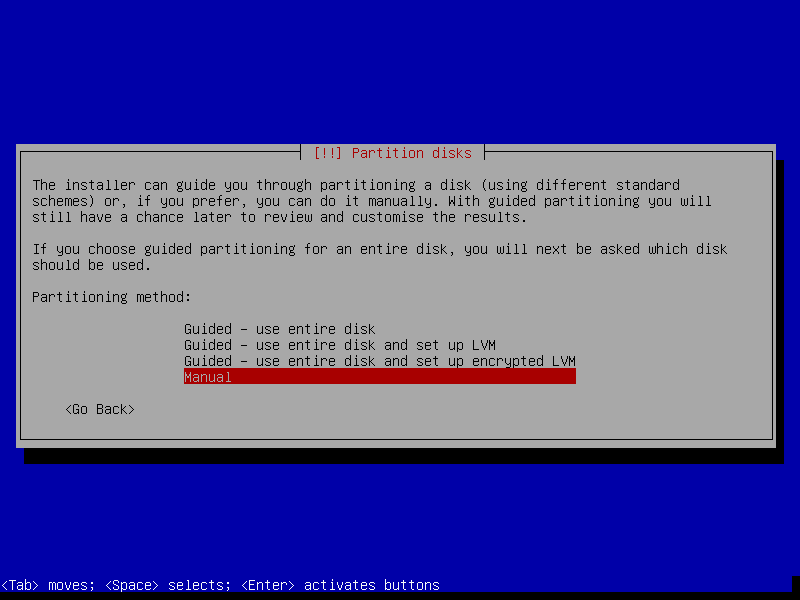
\includegraphics[width=0.8\textwidth, keepaspectratio]{../img/raid install/raid1.png}
    \centering
    \caption{Seleziona partizionamento manuale}

    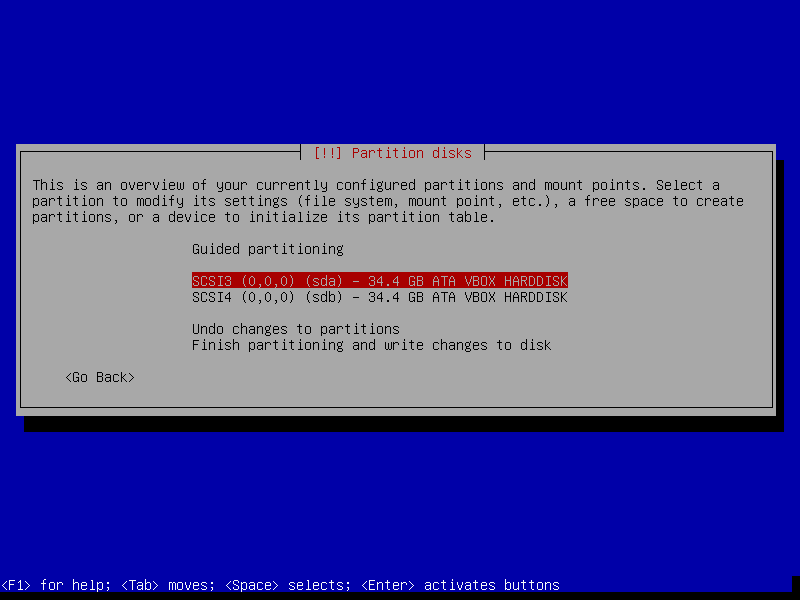
\includegraphics[width=0.8\textwidth, keepaspectratio]{../img/raid install/raid2.png}
    \centering
    \caption{Crea una tabella di partizione vuota sui dischi usati per il RAID1}
\end{figure}

\begin{figure}[H]
    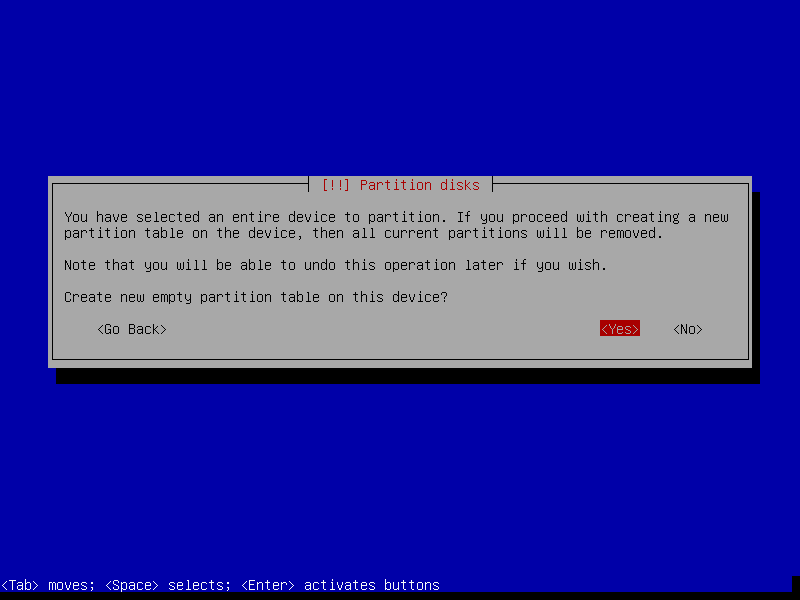
\includegraphics[width=0.8\textwidth, keepaspectratio]{../img/raid install/raid3.png}
    \centering

    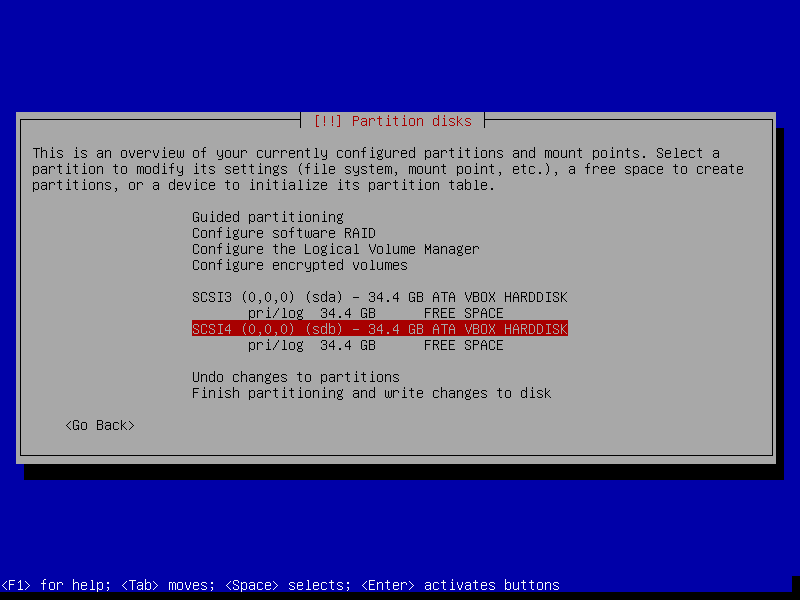
\includegraphics[width=0.8\textwidth, keepaspectratio]{../img/raid install/raid4.png}
    \centering
\end{figure}

\begin{figure}[H]
    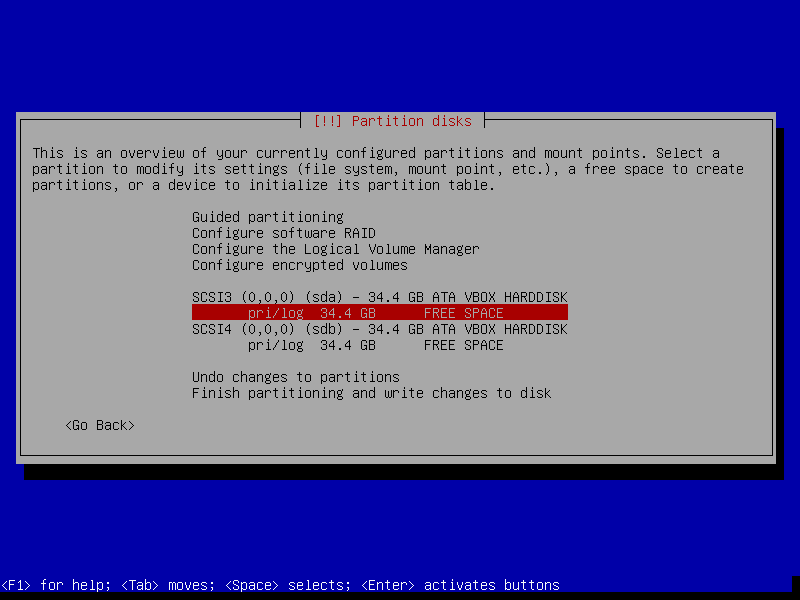
\includegraphics[width=0.8\textwidth, keepaspectratio]{../img/raid install/raid5.png}
    \centering
    \caption{Crea partizione del primo disco}

    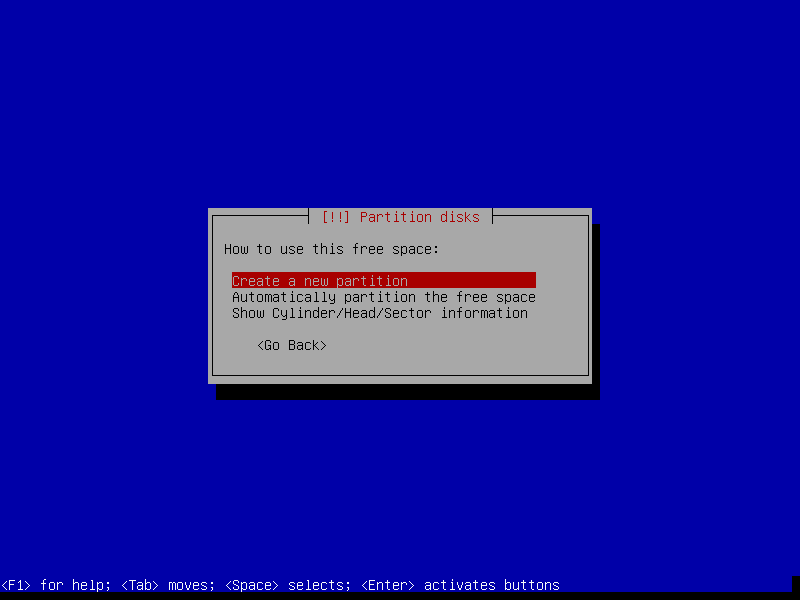
\includegraphics[width=0.8\textwidth, keepaspectratio]{../img/raid install/raid6.png}
    \centering
    \caption{Seleziona partizionamento manuale}
\end{figure}

\begin{figure}[H]
    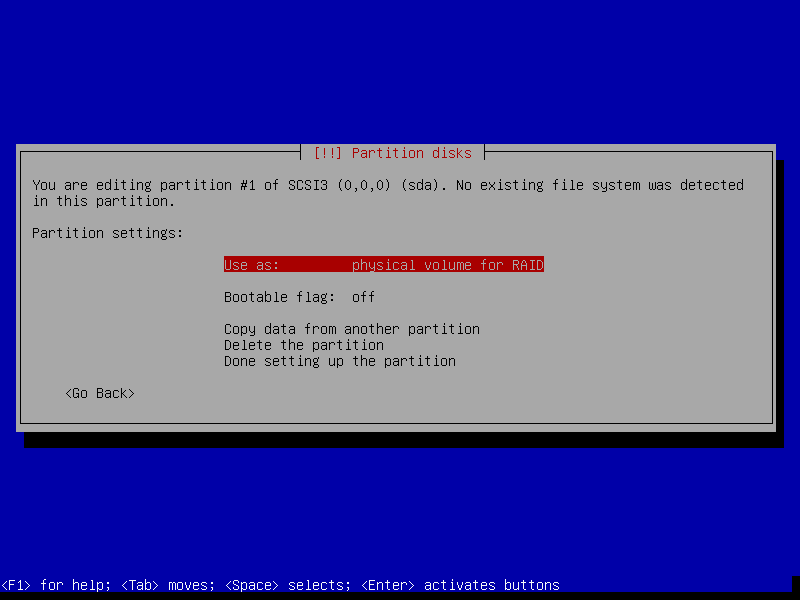
\includegraphics[width=0.8\textwidth, keepaspectratio]{../img/raid install/raid7.png}
    \centering
    \caption{Specificare il tipo della partizione come volume fisico RAID}

    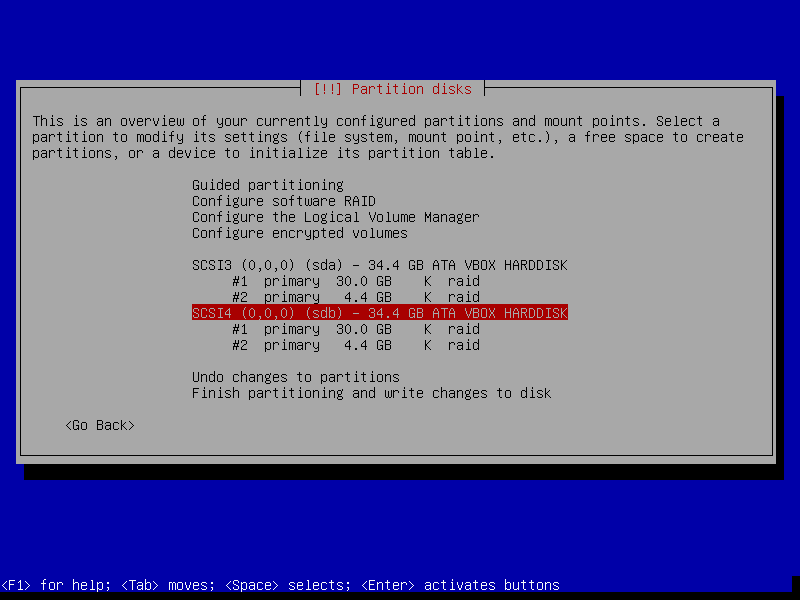
\includegraphics[width=0.8\textwidth, keepaspectratio]{../img/raid install/raid8.png}
    \centering
    \caption{Replicare il processo per il secondo disco}
\end{figure}

\begin{figure}[H]
    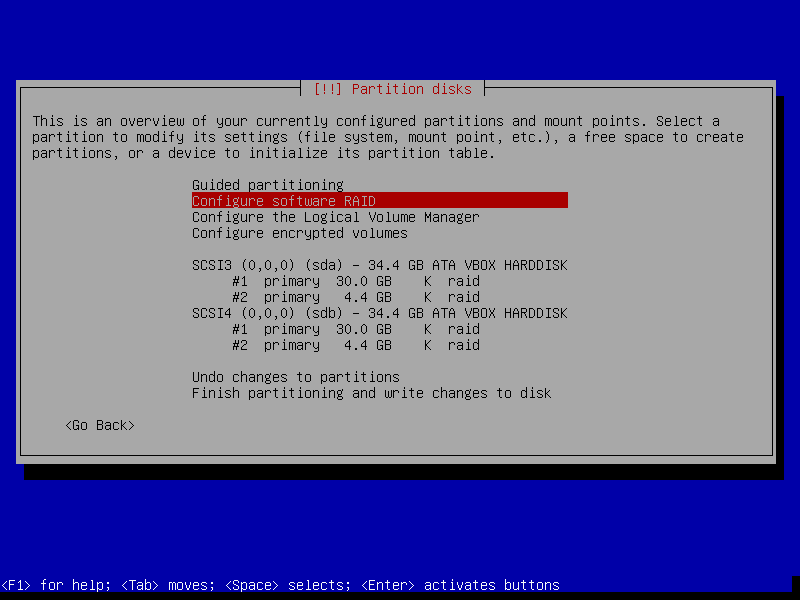
\includegraphics[width=0.8\textwidth, keepaspectratio]{../img/raid install/raid9.png}
    \centering
    \caption{Configurare software RAID}

    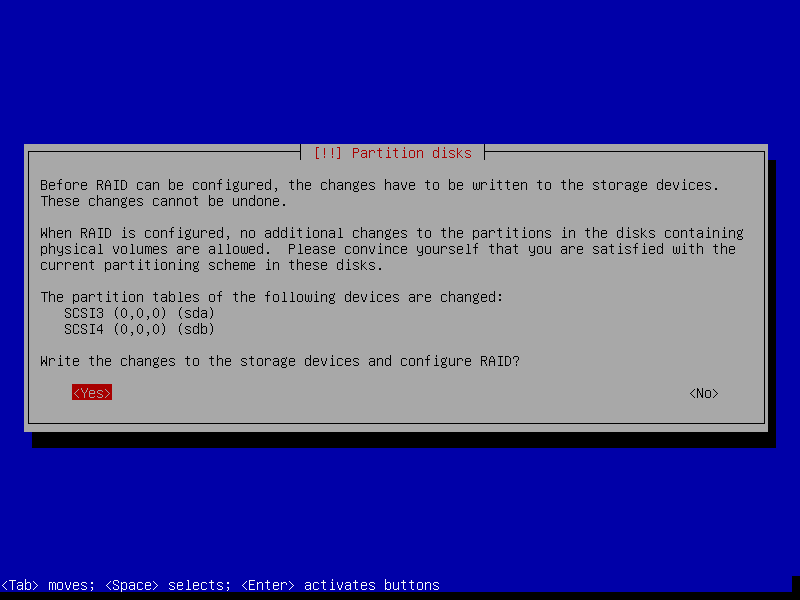
\includegraphics[width=0.8\textwidth, keepaspectratio]{../img/raid install/raid10.png}
    \centering
\end{figure}

\begin{figure}[H]
    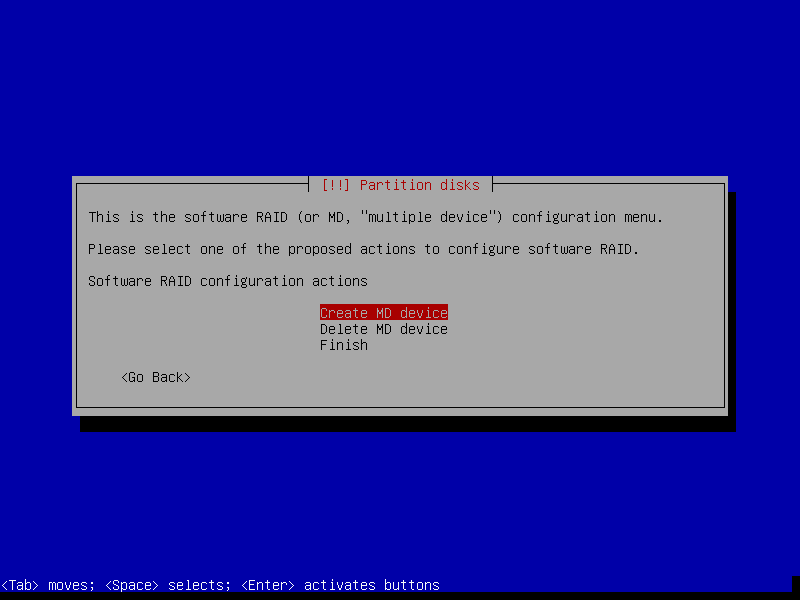
\includegraphics[width=0.8\textwidth, keepaspectratio]{../img/raid install/raid11.png}
    \centering
    \caption{Creare due dispositivi MD per le nuove partizioni}

    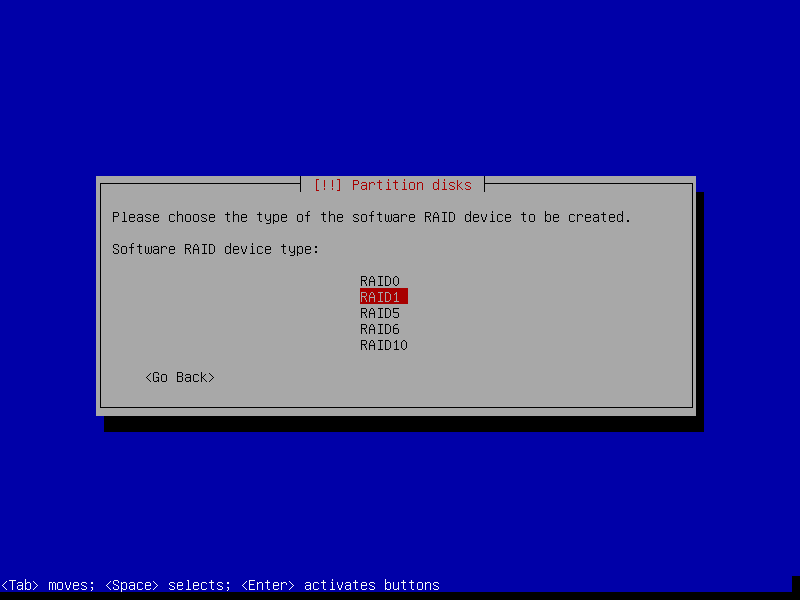
\includegraphics[width=0.8\textwidth, keepaspectratio]{../img/raid install/raid12.png}
    \centering
    \caption{Scegliere livello di RAID}
\end{figure}

\begin{figure}[H]
    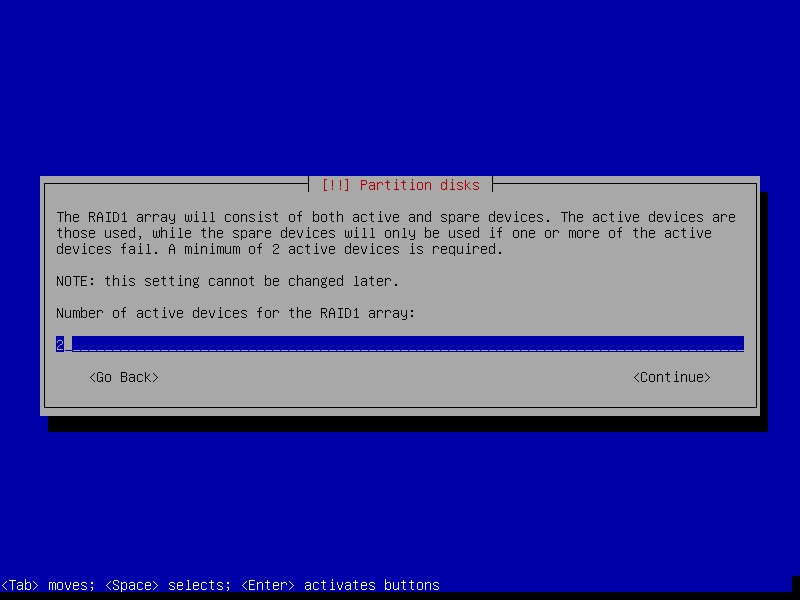
\includegraphics[width=0.8\textwidth, keepaspectratio]{../img/raid install/raid13.png}
    \centering
    \caption{Impostare il numero di dispositivi per l'array}

    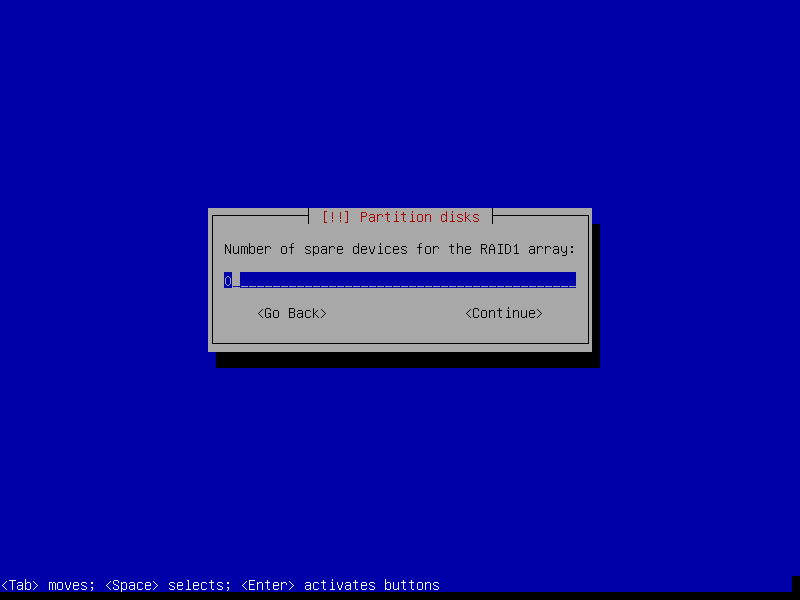
\includegraphics[width=0.8\textwidth, keepaspectratio]{../img/raid install/raid14.png}
    \centering
    \caption{Scegliere il numero di spare devices}
\end{figure}

\begin{figure}[H]
    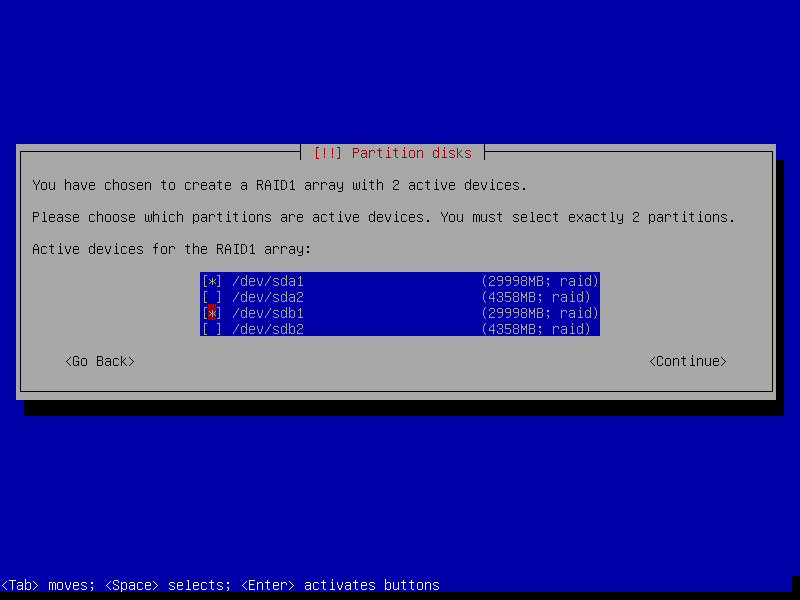
\includegraphics[width=0.8\textwidth, keepaspectratio]{../img/raid install/raid15.png}
    \centering
    \caption{Selezionare i dispositivi attivi}

    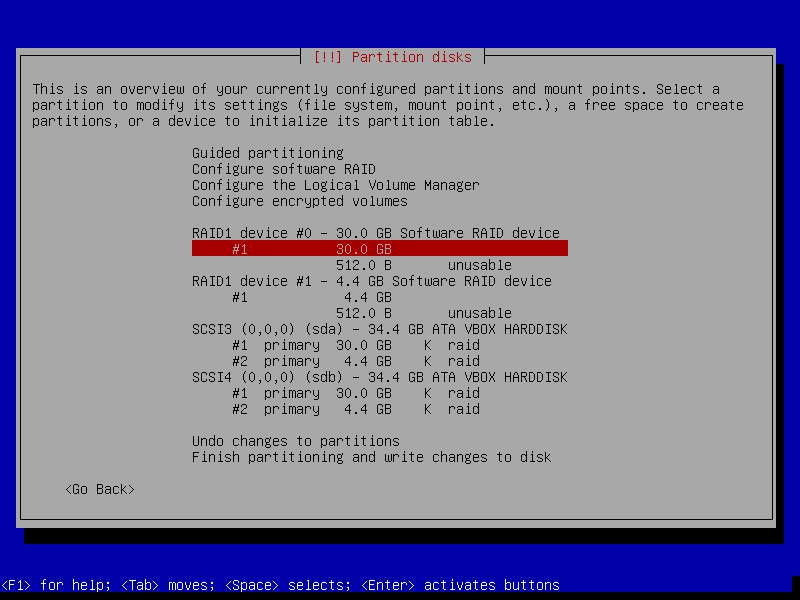
\includegraphics[width=0.8\textwidth, keepaspectratio]{../img/raid install/raid16.png}
    \centering
    \caption{Creare il filesystem di root sul dispositivo RAID}
\end{figure}

\subsection{Configurazione di RAID 5}
\subsection{Creazione e configurazione dell'utenza}
\subsection{Installazione e configurazione di SAMBA}
\subsection{Sistema di alert}



\section{Conclusioni}


\end{document}